\section{Implementation}\label{sect:seapp_implementation}

In this section, we describe the main changes introduced in Android by
\pap.  We first analyze the modifications required to manage policy
modules, both during device boot and at app installation.  We then
describe how the runtime support was realized.

\subsection{Policy compilation}\label{sect:seapp_syst_impl}

\subsubsection{Boot procedure}

Since the introduction of Project Treble \cite{seapp_treble}, policy
files are split among multiple partitions, one for each device
maintainer (i.e., platform, SoC vendor, ODM, and OEM).  This feature
facilitates updates to new versions of Android, separating the Android
OS Framework from the device-specific low-level software written by
the chip manufacturers.  Yet, each time a partition policy (i.e., a
segment) changes, an on-device compilation is required.

The \init process divides its operations in three
stages~\cite{seapp_initstages}: (i) {\em first stage} (early mount),
(ii) \sel setup, and (iii) {\em second stage} (init.rc).  The first
stage mounts the essential partitions (i.e., \dev, \proc, \sys and
\selinuxfsfull), alongside some other partitions specified as early
mounted (since Android 10 using an \fstab file in the first stage
ramdisk, in Android 9 and lower adding fstab entries using device tree
overlays).  Once the required partitions are mounted, \init enters the
SELinux setup.  As the name suggests, this is the stage where \init
loads the \sel policy.  As the \data partition, where policy modules
are stored, is not yet mounted, it is not yet possible to integrate
them with the policy of the system.  Then, as last operation of the
SELinux setup stage, \init re-executes itself to transition from the
initial \kernel domain to the \initdomain domain, entering the second
stage.  As the second stage starts, \init parses the \initrc files and
performs the builtin functions listed there, among them mounting the
\data partition.  Now, the policy modules are available, and we can
produce with \secilc~\cite{seapp_secilccom} (the \sel CIL compiler)
the binary policy consisting of the integration among the system
policy, the \pap macros and the app policy modules.  To trigger the
build and reload of the policy, we implemented a new builtin function,
and modified the \initrc to call this function right after \data is
mounted.  The policy is considered immediately after the \data
partition is available and this ensures that the policy modules are
loaded far before an application starts, making the policy not
bypassable.

Even though most Android devices supporting Android 10 were released
with Treble support and, therefore, execute their \sel setup stage on
the \sepolicy fragments scattered among multiple partitions, \init
still supports the use of a legacy monolithic binary policy.  For
compatibility towards devices using a monolithic binary policy,
additional changes are required, as \pap needs the system policy
written in CIL to be compiled alongside with app modules.  To this
end, we modified the Android build process to push the \sepolicy files
onto the device even for non-Treble devices.  New entries in the
device tree were added to make the policy segments available during
\init \sel setup stage \cite{seapp_early}.

As previously mentioned, we decided to store the policy modules in the
\data partition; even if this choice required us to adapt the boot
procedure of the device, it smoothly integrates \pap with the current
Android design.  In fact, the \data partition is one of the few
writable partitions, it is dedicated to hold the APK the user
installs, as well as their dedicated data directories and, therefore,
it represents the best option to contain also the app policy modules.
Moreover, whenever a user performs a factory reset, Android
automatically wipes the \data partition, removing the customization
the user made to the device configuration, including the apps.  By
placing the app policy modules and the apps into the same partition, a
factory reset removes the policy modules as well.

\begin{figure}[h]
	\begin{center}
		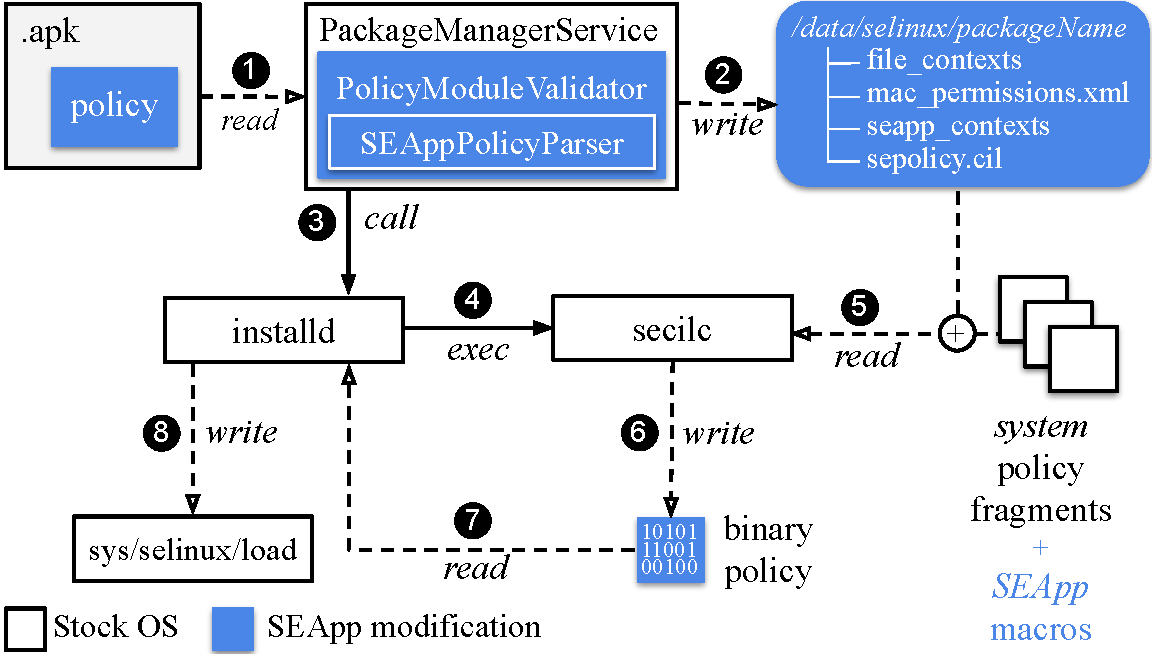
\includegraphics[width=0.8\columnwidth]{chapters/seapp/figs/app_installation}
	\end{center}
	\caption{\label{fig:seapp_install} Installation process}
\end{figure}

\subsubsection{App installation}

As introduced in Section~\ref{subsect:seapp_structure}, the developer
willing to define its own policy module is expected to load it in the
app package.  At app installation, the \pms~\cite{seapp_pmsserva}
inspects the APK to identify whether or not the current installation
involves a policy module, by looking for the \apkpolicydir directory
at the root of the archive.  When the app has a policy module attached
to it (see Figure~\ref{fig:seapp_install}), the \pms extracts it
(\blackcircle{1}) and uses our \textit{PolicyModuleValidator} to
verify the respect of all the constraints on \sepolicy (through the
{\em SEAppPolicyParser}, Section \ref{sect:seapp_lang}) and on the
configuration files (Section \ref{sect:seapp_config}).  In case of a
violation of the constraints, the app installation stops.  Otherwise,
the policy module is stored within \dataselinux, in a dedicated
directory identified by the package name (\blackcircle{2}).  Then, the
\pms invokes \installd~\cite{seapp_installdid} through the {\em
  Installer} to trigger the policy compilation with an exec call to
the \secilc program (\blackcircle{3}, \blackcircle{4}).  {\em Secilc}
reads the system \sepolicy fragments, the \pap macros and the
\sepolicy fragments of the app policy modules in the \dataselinux
directory (\blackcircle{5}), and builds the binary policy
(\blackcircle{6}).  When the \secilc execution returns and no
compilation errors have been raised, the binary policy is then read by
\installd (\blackcircle{7}) and loaded with \loadpolicy, which writes
the \texttt{sys/selinux/load} file (\blackcircle{8}).

To load the policy files after \init, the implementation of SELinux in
Android has been slightly modified.  In particular, we modified the
policy loading function within \libselinux (function \loadpolicy), and
changed the system policy to allow \installd to load the app policy
module.

As for the policy configuration files, some changes were introduced to
load the application \filecontexts, \seappcontexts and
\macpermissions.  {\em SELinuxMMAC}~\cite{seapp_mmacsel}, i.e., the
class responsible for loading the appropriate {\tt mac\textunderscore
  pe}- \newline {\tt rmissions.xml} file and assigning \seinfo values
to apks, was modified to load the new \macpermissions specified within
the app policy module.  The loading of \filecontexts and
\seappcontexts was configured to treat system and app configuration
files apart.  So, \pap-enhanced applications will load exclusively
their configuration files, whereas the loading of system's and other
apps' configuration files is not needed since their use is prohibited.
System services and daemons, instead, load the base system
configurations once, and then load the app policy module specific
configuration files as they are needed.  An example of this are
\zygote and \restorecon services, which need to retrieve at runtime
\seappcontexts and \filecontexts, respectively (see
Section~\ref{sect:seapp_app_runtime}).

Our implementation also supports the uninstallation of \pap apps.  The
regular uninstallation process is extended with a step where the
global policy is recompiled, in order to remove the impact of old
modules on the overall binary policy.  With reference to application
updates, the native \installd runs with the necessary permission to
remove and apply new file types based on the content of the
\filecontexts.

\subsection{Runtime support}\label{sect:seapp_app_runtime}

In addition to the steps described above, other aspects have to be
considered in order to extend SELinux support at the application
layer.

\begin{figure}[h]
  \centering
  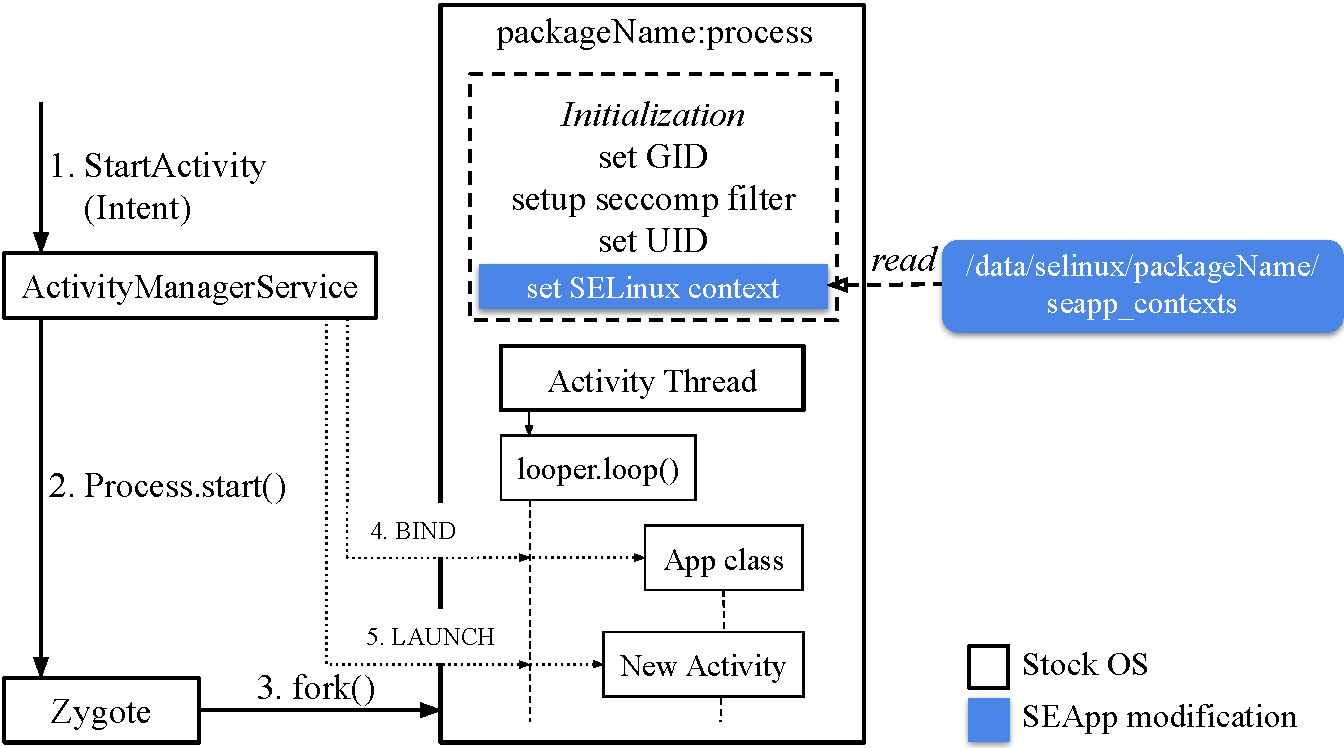
\includegraphics[width=0.8\columnwidth]{chapters/seapp/figs/app_launch}
  \caption{\label{fig:seapp_runtime} Application launch}
\end{figure}

\subsubsection{Processes}

Android application design is based on components.  Each of them lives
inside a process, and can be seen as an entry point through which the
system or the user can enter the app.

To activate a component, an asynchronous message called intent,
containing both the reference to the target component and parameters
needed for its execution, has to be created.  The intent is then
routed by the system to the {\em
  ActivityManagerService}~\cite{seapp_activitymanserv} via {\em Binder
  IPC}.  Before delivering the intent request to the target component,
the {\em ActivityManagerService} checks if the process in which the
target component should be executed is already running; if not, the
native service called \zygote~\cite{seapp_zygoterfi} is executed.  Its
role is to spawn and correctly setup the new application process.  To
achieve this, it first replicates itself by performing a fork, then,
using the input provided by the {\em ActivityManagerService} (namely,
package name, \seinfo, {\tt android:process}, etc.), it starts
configuring the process GID, the {\em seccomp} filter, the UID and
finally the \sel security context.  We adapted the final configuration
step, forcing \zygote to set the security context based on the
\seappcontexts located at {\tt \dataselinuxdir} (i.e., the one
provided by the developer for her app).  Process name is used to
assign the proper context to the process when it starts, before the
logic of the process kicks in.  In case the developer did not specify
a domain, then \zygote uses the system \seappcontexts as fallback.
After the correct labeling, the {\em ActivityManagerService} finishes
the configuration by binding the application class, launching the
component, and finally delivering the intent message.
Figure~\ref{fig:seapp_runtime} details the process.

This implementation design offers several benefits, including backward
compatibility, support for all components, and ease of use.
Indeed, a developer who wants to use our solution only has to
configure some files; changes in the application code are reduced to a
minimum, thus facilitating the introduction of SELinux in already
existing apps.

In our study we have also explored other design alternatives, in which
the developer could explicitly state a domain transition in the code,
wherever she needs it.  Although this category of solutions would give
the developers more control over domain transitions, it also has some
drawbacks.  First, the developer would be expected to enforce the
isolation among source and target domains managing the multi-threaded
scenario, and second, this design implies granting too many
permissions to the app (e.g., \dyntransition, \setcurrent and
read/write access to \selinuxfs).  Moreover, such solution would
introduce a new Android API, that would be quite delicate and, if not
used correctly, it might be difficult to control.

\begin{figure}[t]
  \begin{center}
    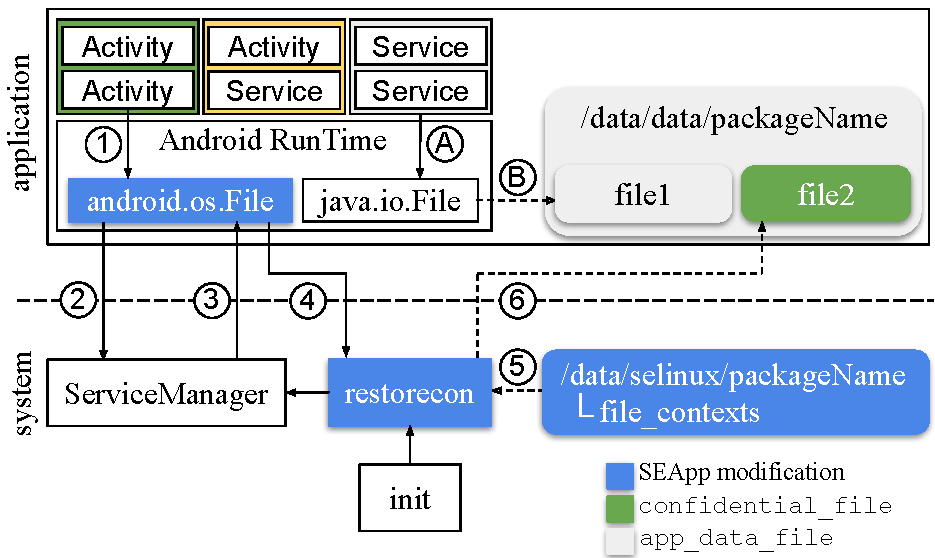
\includegraphics[width=0.8\columnwidth]{chapters/seapp/figs/restorecon_service}
  \end{center}
  \caption{\label{fig:seapp_restorecon} File relabeling}
\end{figure}


\subsubsection{Files}\label{sect:seapp_impl_files}

Android applications aiming to create a file can use the {\tt
  java.io.File} abstraction.  Each file creation request that is
generated is captured by the Android Runtime
(ART)~\cite{seapp_androruntime}, and then converted into the
appropriate syscall.  The result is the creation of the target file,
to which a security context inherited from the parent directory is
assigned (see flow \whitecircle{A}, \whitecircle{B} of
Figure~\ref{fig:seapp_restorecon}).  Since Android 9, the separation
between files of different apps is enforced at MAC level (a unique
context based on UID and \sel category is assigned); however, all the
files stored in the same app folder are labeled with the \appdatafile
type.

To make the most out of \sel, \pap complements Android with the
implementation of a new service, which we called \restorecon (to
recall the \sel \restoreconc tool).  The \restorecon service is
spawned by {\em init} at boot, and works in its own \sel domain.  Its
role is to create and label files as specified by the developer in the
local \filecontexts.  To ease development, we implemented the new {\tt
  android.os.File} abstraction, which exposes an interface equal to
that of {\tt java.io.File}, and transparently handles the call to our
service.  Figure~\ref{fig:seapp_restorecon} details the new control
flow.  A component running in a \pap-enhanced process (highlighted in
green in Figure~\ref{fig:seapp_restorecon}) invokes {\tt
  android.os.file}, and triggers a new file creation request
(\whitecircle{1}).  The new API first interacts with the {\em
  ServiceManager} (\whitecircle{2}) to get a handle of the \restorecon
service (\whitecircle{3}), then it interacts with the service using
the AIDL~\cite{seapp_aaidl} interface we defined for it, informing the
\restorecon of the target path (\whitecircle{4}).  The \restorecon
service verifies whether the caller is the legitimate owner of the
path, it reads the \filecontexts file located at \dataselinuxdir
(\whitecircle{5}), and finally it creates the target file enforcing
the correct labeling (\whitecircle{6}).

We also investigated three other implementation approaches: (i) change
of the default security context inheritance behavior for the {\em
  ext4} filesystem, (ii) execution of the \sel \restorecon operation
by the app, once the file is successfully created, and (iii) use of
\restorecond~\cite{seapp_restorecondd}.  The first option would change
the default behavior system-wide.  As it might cause compatibility
issues, we decided not to choose it.  The second option is not ideal
from a security standpoint, as it requires to grant the application
too many permissions (e.g., \relabelfrom, \relabelto, as well as
read/write access to \selinuxfs to check the validity of the \sel
context).  The third option refers to the use of \restorecond, a
system daemon that watches (inodes of) a configurable list of files
and checks that they are labeled as stated in the system
\filecontexts.  Although it may realize the control, \restorecond was
meant for a few system files, therefore its performance would hardly
scale, especially considering that \pap needs to manage all files
created by \pap-aware apps.  Another major issue is that this approach
is exposed to race conditions, because there is a delay between file
creation and its relabeling.

\begin{figure}[h]
	\centering
  \subfloat{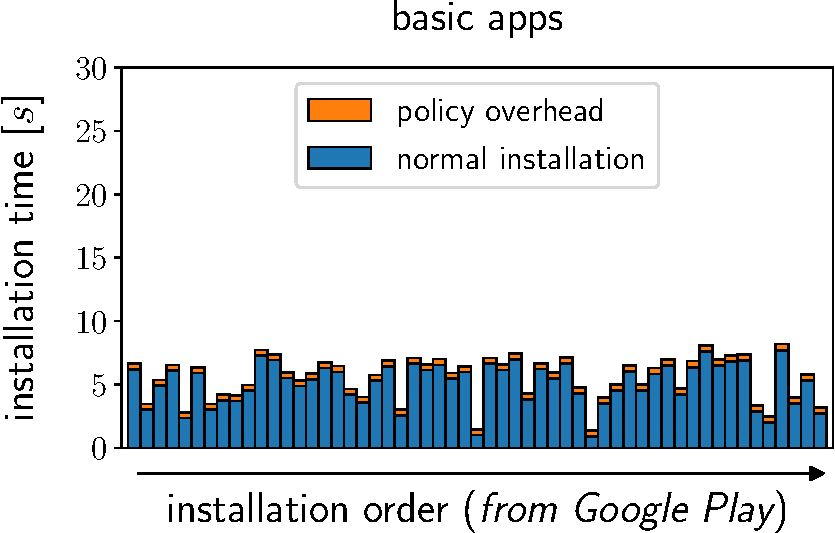
\includegraphics[width=185pt]{chapters/seapp/data/three_kinds_basic}}        
  \hfill
  \subfloat{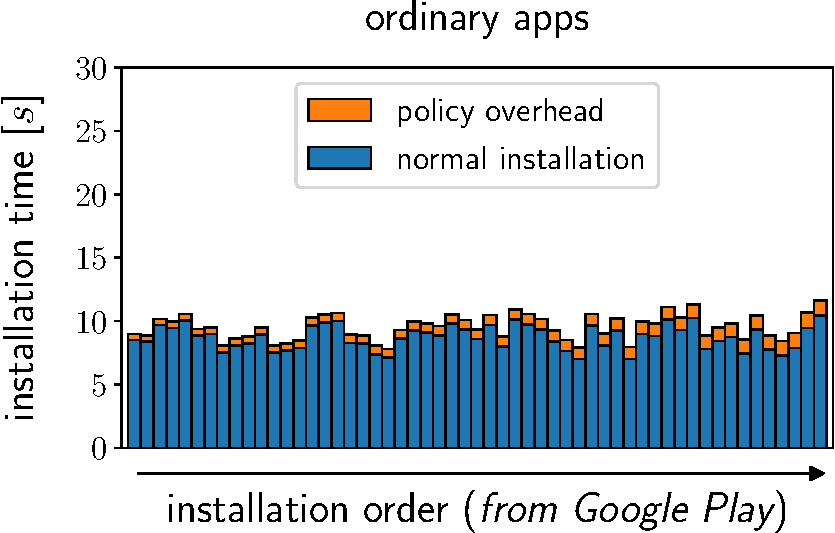
\includegraphics[width=185pt]{chapters/seapp/data/three_kinds_ordinary}}
  \\
  \subfloat{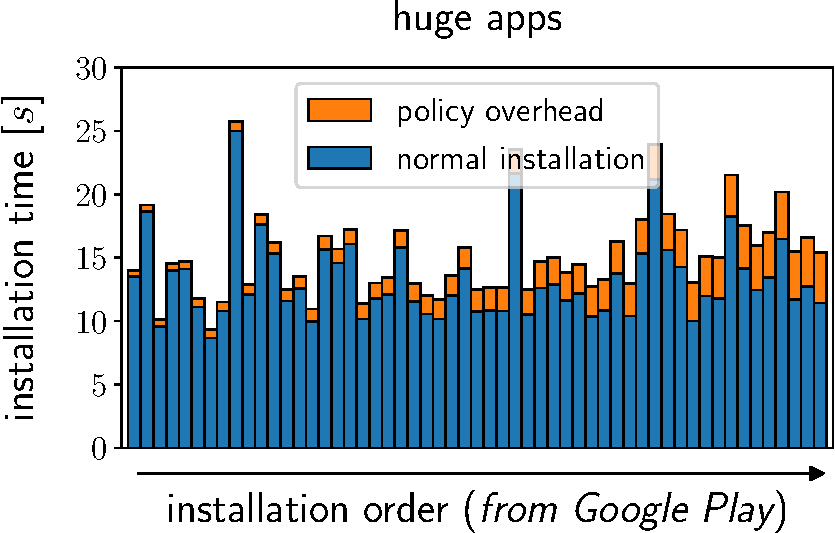
\includegraphics[width=185pt]{chapters/seapp/data/three_kinds_huge}}
	\caption{\label{fig:seapp_three_kinds} Installation time overhead for apps with different complexity}
\end{figure}      


%%% Local Variables: 
%%% mode: latex
%%% TeX-master: "../../../main.tex"
%%% reftex-default-bibliography: "../../../bib/biblio.bib"
%%% End: